\documentclass[12pt,a4paper]{article}

\usepackage[left=30mm, right=15mm, top=20mm, bottom=20mm]{geometry}
\usepackage[T1]{fontenc}
\usepackage[utf8]{inputenc}
\usepackage{times}
\usepackage{graphicx}
\usepackage{booktabs}
\usepackage{longtable}
\usepackage{array}
\usepackage{ragged2e}
\usepackage{hyperref}
\usepackage{enumitem}
\usepackage{float}
\usepackage{listings}
\usepackage{xcolor}
\usepackage{tabularx}
\usepackage{caption}
\usepackage{tikz}
\usetikzlibrary{arrows.meta, positioning, shapes.geometric, fit, calc}

\hypersetup{
    colorlinks=true,
    linkcolor=black,
    urlcolor=blue,
    citecolor=black,
}

\setlength{\parindent}{1.25cm}
\setlength{\parskip}{0.4em}
\renewcommand{\baselinestretch}{1.5}
\newcolumntype{Y}{>{\RaggedRight\arraybackslash}X}

\begin{document}

\section*{Chapter 3}
\addcontentsline{toc}{section}{Chapter 3: Design and Methodology}

\begin{center}
    {\Large \textbf{Design and Methodology}}
\end{center}

\subsection{Development Process}

The development of the Qamqorshy platform followed an Agile methodology with short, practical iterations. This approach suited a student team because it kept the project flexible and allowed the team to react quickly when requirements changed, technical issues appeared, or interface decisions needed refinement. Instead of trying to design everything in one attempt, the team built the system step by step, checked the result after each cycle, and improved the next version based on what they learned. That rhythm made the work feel manageable. It also helped the team keep the product aligned with the original idea rather than drifting into unnecessary features.

The project itself was completed by \textbf{[Insert Team Name Here]}. The team divided work by responsibility, but the process stayed collaborative throughout the whole project. Frontend tasks, backend tasks, design tasks, and testing tasks moved in parallel. Regular discussions helped the team resolve blockers early, especially when one feature depended on another. In practice, this meant the user interface could evolve while API endpoints were still being refined, and the database could grow without forcing a full redesign every time a new field was needed.

\subsubsection{Problem Statement and Initial Research}

Qamqorshy started from a very specific gap in the Kazakhstan digital services market. While there are large local platforms such as \texttt{naimi.kz} and \texttt{olx.kz} where people can look for many kinds of services, they do not offer a focused, trustworthy environment for caregiving. During the initial research, the team examined how users could search for pet sitters, child caregivers, and elderly support on those platforms. The result was revealing. In many cases, search results showed only two or three suitable profiles. Even more importantly, those profiles were usually universal workers who offered cleaning, delivery, repair, and caregiving at the same time. That pattern suggested a clear problem: caregiving was not their main professional service.

This situation matters because caregiving is not just another household task. When a family looks for someone to care for a child, an elderly relative, or a pet, trust becomes the central factor. Users do not simply need ``someone available.'' They need a person with a relevant profile, clear experience, visible reviews, understandable pricing, and a safe communication flow. General service marketplaces do not emphasize those things strongly enough. They are broad by design. Qamqorshy, in contrast, was designed as a narrow but deeper platform dedicated to caregiving.

The research phase therefore focused on three conclusions. First, Kazakhstan lacks a specialized caregiving platform that brings different care categories together in one system. Second, existing marketplace listings are too fragmented and too generic to inspire confidence. Third, any new solution in this area must address trust directly through verification, transparency, structured booking, and controlled communication. These findings shaped both the functional requirements and the system architecture of the platform.

\subsubsection{Requirements Gathering}

After defining the problem space, the team translated the research into concrete requirements. The first group of requirements described the essential behavior of the platform. The system had to support three user roles: client, caregiver, and administrator. Clients needed to register, browse caregivers, create bookings, communicate with assigned caregivers, monitor service quality, and leave reviews. Caregivers needed to create accounts, complete profiles, upload verification documents, receive or accept bookings, negotiate price, exchange messages, and publish progress updates during active sessions. Administrators needed to monitor the platform, verify caregiver documents, and view summary statistics.

The team also identified several non-functional requirements early in the process. The platform had to provide a simple and understandable interface because many users would not be technical. It had to support multiple languages because a caregiving product in Kazakhstan should not depend on one language only. The system had to protect private user data, especially authentication data and messages. Finally, the project needed a modular technical structure so the frontend and backend could evolve independently during development.

To keep the scope realistic, the team prioritized the features that directly supported the main service flow. Those features included authentication, profile management, caregiver listing, booking creation, booking negotiation, messaging, quality updates, reviews, multilingual support, and administrator tools. Features outside the core flow were left for future expansion.

\subsubsection{Agile Planning and Sprint Workflow}

The team organized the work in short sprints. Each sprint focused on a small set of features that could be designed, implemented, and tested together. This structure reduced confusion because everyone knew what the immediate goal was. It also reduced rework. If a decision turned out to be weak, the team could correct it in the next sprint instead of discovering the problem near the end of the whole project.

Task tracking was handled with \textbf{[Insert Project Management Tool Here]} using a Kanban-style board. The board included columns such as \textit{To Do}, \textit{In Progress}, \textit{Review}, and \textit{Done}. This setup helped the team see bottlenecks quickly. If too many tasks gathered in review, then integration work had to become the priority. If backend tasks blocked frontend work, the team could reprioritize endpoints before continuing with presentation details.

Communication happened through \textbf{[Insert Communication Tool Here]} and regular meetings. These meetings were especially useful when frontend and backend contracts had to be synchronized. For example, the booking workflow included status transitions and price negotiation data, so both sides of the application had to agree on how those values would be named, updated, and displayed. Short and frequent communication kept those details consistent.

\subsubsection{Design Validation and Iterative Refinement}

The project did not move directly from idea to final implementation. Before writing a large amount of code, the team explored interface structure, user flows, and component relationships. This design phase included page planning, role-based navigation, color choices, and database thinking. Instead of treating design as decoration, the team used it as a practical tool for reducing confusion during development.

Several parts of the platform changed during iteration. The booking flow became clearer after the team decided to keep the steps short and structured. The messaging system became safer once it was tied to active bookings rather than allowing arbitrary direct messages. The caregiver verification logic also improved during iteration because profile updates and document submission needed to trigger a pending verification state instead of relying on manual database edits. These refinements are a good example of why an iterative process worked well for this project. Each cycle made the system more coherent.

\subsection{Design and Methodology}

\subsubsection{System Architecture}

Qamqorshy uses a client-server architecture with a clear separation between the presentation layer, the application layer, and the data layer. The frontend is implemented with Next.js and React. The backend is implemented with FastAPI and Python. Persistent data is stored in PostgreSQL through SQLAlchemy models and Alembic migrations. This architecture was chosen because it allowed the team to develop the interface and the business logic in parallel while keeping the database layer consistent and maintainable.

The frontend handles page rendering, navigation, user interactions, and API integration. The backend is responsible for authentication, access control, business rules, and database operations. The database stores all persistent entities such as users, caregiver profiles, bookings, messages, reviews, and quality updates. This division of responsibilities made the project easier to reason about. It also made debugging easier because the team could isolate whether a problem came from the interface, the API, or the schema.

\begin{figure}[H]
\centering
\resizebox{\textwidth}{!}{
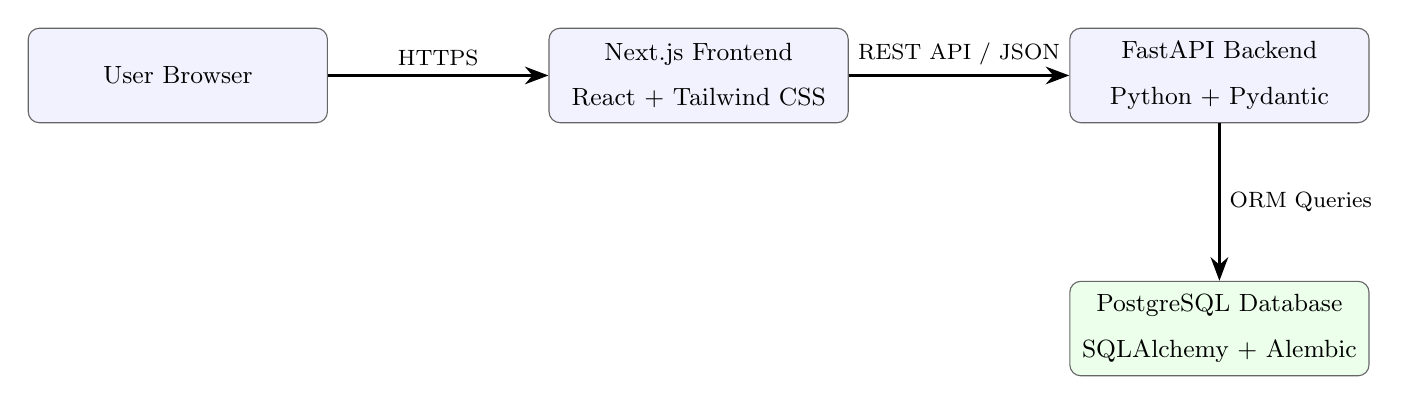
\begin{tikzpicture}[
    box/.style={rectangle, draw=black!60, rounded corners=4pt, minimum width=3.8cm, minimum height=1.2cm, align=center, fill=blue!5, font=\small},
    db/.style={rectangle, draw=black!60, rounded corners=4pt, minimum width=3.8cm, minimum height=1.2cm, align=center, fill=green!8, font=\small},
    arr/.style={-{Stealth[length=3mm]}, thick}
]
\node[box] (browser) {User Browser};
\node[box, right=2.8cm of browser] (frontend) {Next.js Frontend\\React + Tailwind CSS};
\node[box, right=2.8cm of frontend] (backend) {FastAPI Backend\\Python + Pydantic};
\node[db, below=2cm of backend] (database) {PostgreSQL Database\\SQLAlchemy + Alembic};

\draw[arr] (browser) -- node[above, font=\footnotesize]{HTTPS} (frontend);
\draw[arr] (frontend) -- node[above, font=\footnotesize]{REST API / JSON} (backend);
\draw[arr] (backend) -- node[right, font=\footnotesize]{ORM Queries} (database);
\end{tikzpicture}
}
\caption{High-level architecture of the Qamqorshy platform}
\label{fig:qamqorshy-architecture}
\end{figure}

One practical advantage of this architecture lies in how authentication works. The frontend relies on a session cookie, while the backend validates the token and returns only the data the current user is allowed to see. That design reduced duplication and made role-based behavior more reliable across the platform.

\subsubsection{Technology Stack}

The selected technology stack balanced development speed, readability, and practical reliability. Table \ref{tab:stack} summarizes the main technologies used in the project and the reason each one mattered.

\begin{table}[H]
\centering
\caption{Technology stack of the Qamqorshy platform}
\label{tab:stack}
\small
\begin{tabularx}{\textwidth}{>{\RaggedRight\arraybackslash}p{2.5cm} >{\RaggedRight\arraybackslash}p{2.7cm} Y}
\toprule
\textbf{Layer} & \textbf{Technology} & \textbf{Purpose} \\
\midrule
Frontend & Next.js 16 & Server-rendered React application with file-based routing and structured page organization. \\
Frontend UI & React 19 & Component-based user interface development. \\
Styling & Tailwind CSS 4 & Utility-first styling for responsive and consistent design. \\
Animation/UI & GSAP, Radix UI, Shadcn UI & Motion effects and reusable accessible interface primitives. \\
Validation on client & Zod & Structured validation of form data and typed client-side contracts. \\
Backend & FastAPI & High-performance Python web framework with clear API definitions. \\
Backend validation & Pydantic 2 & Request and response validation for API safety and consistency. \\
ORM & SQLAlchemy 2 & Object-relational mapping between Python models and PostgreSQL tables. \\
Migrations & Alembic & Versioned database migration management. \\
Database & PostgreSQL & Persistent relational storage for platform data. \\
Security & bcrypt, python-jose & Password hashing and JWT token generation. \\
Version control & Git & Collaborative source code management. \\
\bottomrule
\end{tabularx}
\normalsize
\end{table}

This stack worked well for a student software project because it gave the team modern development tools without introducing unnecessary complexity. FastAPI, for example, automatically validated request data. That feature saved time and reduced bugs. Next.js, on the other hand, gave the frontend a clean page structure and simple routing conventions. Together, these tools created a development environment that was productive and relatively easy to maintain.

\subsubsection{Project Structure}

The codebase is divided into two major parts: the frontend project and the backend project. This split mirrors the system architecture and keeps responsibilities separate.

The frontend project contains the application pages, shared UI components, widgets, authentication helpers, API utilities, and translation logic. Important routes include the landing page, login page, registration page, user dashboard, booking page, profile page, caregiver listing, caregiver details, messages page, quality monitoring page, reviews page, and administrator panel.

The backend project is organized around API route modules, database models, schema definitions, and core configuration. The route layer includes dedicated modules for authentication, users, profiles, caregivers, bookings, messages, reviews, language selection, quality updates, administrator statistics, and verification documents. This modular structure improved readability because each route file focused on one domain area instead of mixing unrelated behavior in a single place.

\begin{figure}[H]
\centering
\resizebox{0.92\textwidth}{!}{
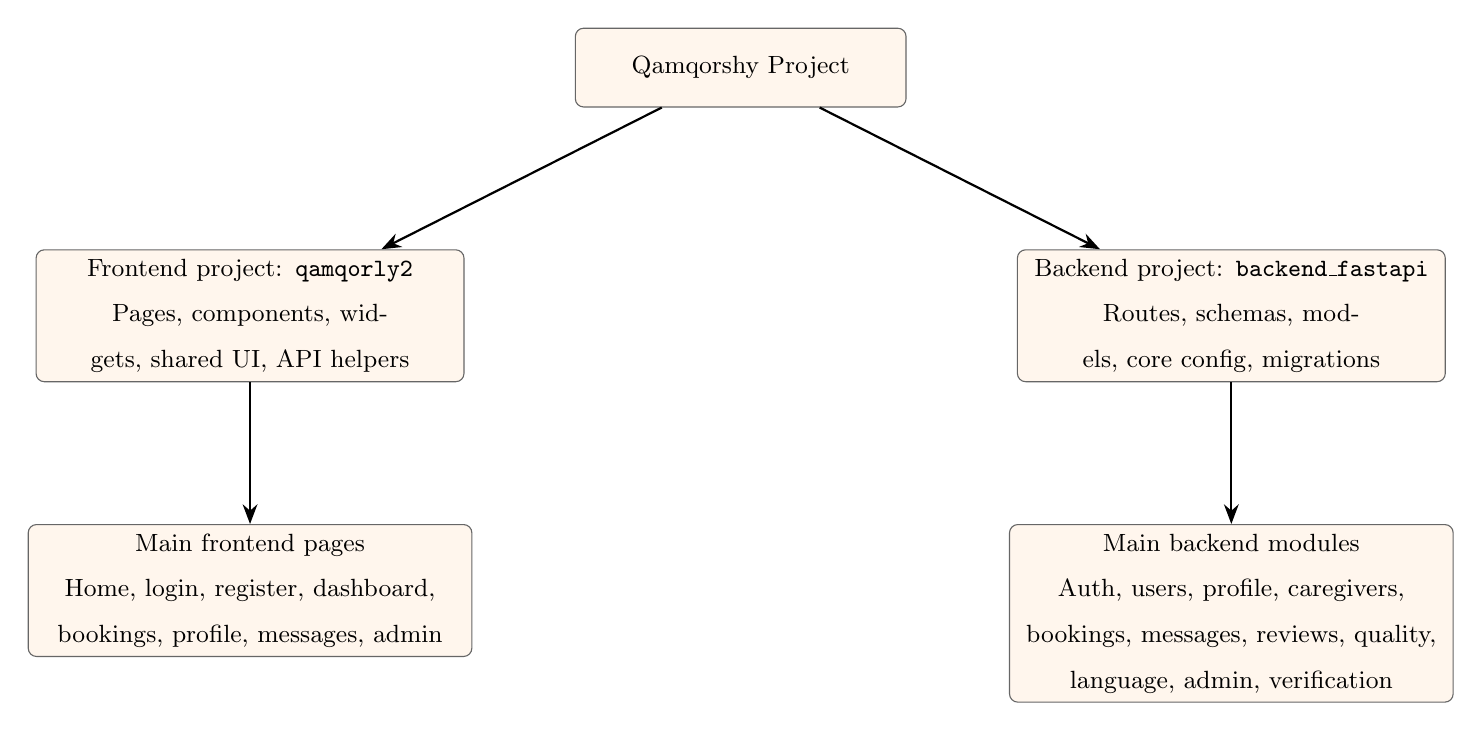
\begin{tikzpicture}[
    folder/.style={rectangle, draw=black!60, rounded corners=3pt, fill=orange!7, minimum width=4.2cm, minimum height=1cm, align=center, font=\small},
    arr/.style={-{Stealth[length=2.5mm]}, thick}
]
\node[folder] (root) {Qamqorshy Project};
\node[folder, below left=1.8cm and 1.4cm of root, text width=5.2cm] (front) {Frontend project: \texttt{qamqorly2}\\Pages, components, widgets, shared UI, API helpers};
\node[folder, below right=1.8cm and 1.4cm of root, text width=5.2cm] (back) {Backend project: \texttt{backend\_fastapi}\\Routes, schemas, models, core config, migrations};
\node[folder, below=1.8cm of front, text width=5.4cm] (frontpages) {Main frontend pages\\Home, login, register, dashboard, bookings, profile, messages, admin};
\node[folder, below=1.8cm of back, text width=5.4cm] (backmodules) {Main backend modules\\Auth, users, profile, caregivers, bookings, messages, reviews, quality, language, admin, verification};

\draw[arr] (root) -- (front);
\draw[arr] (root) -- (back);
\draw[arr] (front) -- (frontpages);
\draw[arr] (back) -- (backmodules);
\end{tikzpicture}
}
\caption{Simplified project structure of Qamqorshy}
\label{fig:qamqorshy-structure}
\end{figure}

\subsubsection{User Roles and UML-Oriented Design}

The platform revolves around three system roles. Each role has a different goal and a different set of allowed actions.

\begin{itemize}[leftmargin=1.5cm]
    \item \textbf{Client} registers, manages a personal profile, browses caregivers, creates bookings, negotiates with caregivers, exchanges booking-scoped messages, reads quality updates for assigned bookings, and leaves reviews after completed bookings.
    \item \textbf{Caregiver} registers as a specialist, defines service categories and hourly rate, uploads verification documents, accepts or negotiates bookings, communicates with assigned clients, and posts quality updates for assigned non-completed bookings.
    \item \textbf{Administrator} monitors platform statistics, reviews caregiver verification documents, and can also update a caregiver's overall verification status directly through the administrator route.
\end{itemize}

\begin{figure}[H]
\centering
\resizebox{0.95\textwidth}{!}{
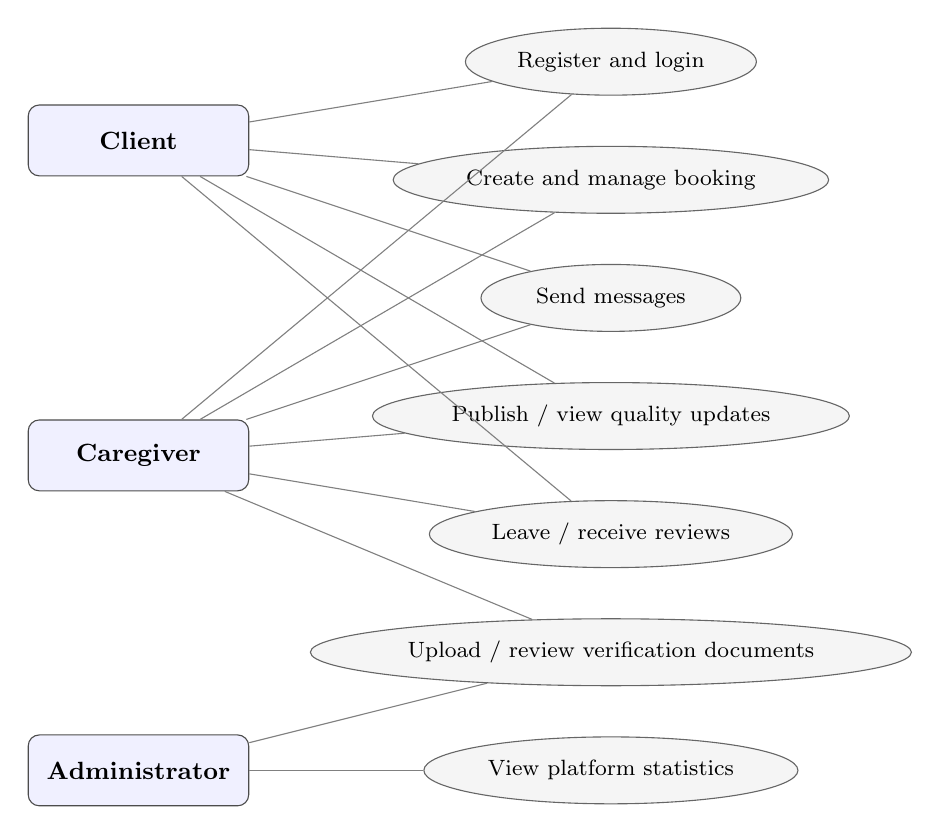
\begin{tikzpicture}[
    actor/.style={rectangle, draw=black!70, rounded corners=4pt, minimum width=2.8cm, minimum height=0.9cm, align=center, fill=blue!6, font=\small\bfseries},
    usecase/.style={ellipse, draw=black!60, minimum width=3.3cm, minimum height=0.85cm, align=center, fill=gray!8, font=\footnotesize},
    line/.style={draw=black!50}
]
\node[actor] (client) at (0,0) {Client};
\node[actor] (caregiver) at (0,-4) {Caregiver};
\node[actor] (admin) at (0,-8) {Administrator};

\node[usecase] (register) at (6,1) {Register and login};
\node[usecase] (booking) at (6,-0.5) {Create and manage booking};
\node[usecase] (message) at (6,-2) {Send messages};
\node[usecase] (quality) at (6,-3.5) {Publish / view quality updates};
\node[usecase] (review) at (6,-5) {Leave / receive reviews};
\node[usecase] (verify) at (6,-6.5) {Upload / review verification documents};
\node[usecase] (stats) at (6,-8) {View platform statistics};

\draw[line] (client) -- (register);
\draw[line] (client) -- (booking);
\draw[line] (client) -- (message);
\draw[line] (client) -- (quality);
\draw[line] (client) -- (review);

\draw[line] (caregiver) -- (register);
\draw[line] (caregiver) -- (booking);
\draw[line] (caregiver) -- (message);
\draw[line] (caregiver) -- (quality);
\draw[line] (caregiver) -- (review);
\draw[line] (caregiver) -- (verify);

\draw[line] (admin) -- (verify);
\draw[line] (admin) -- (stats);
\end{tikzpicture}
}
\caption{UML-style overview of system roles and main use cases}
\label{fig:qamqorshy-usecases}
\end{figure}

This role separation is also reflected in the backend access rules. Clients cannot verify caregivers. Caregivers cannot access administrator statistics. Administrators do not use the same profile-editing flow as regular users. These boundaries helped the team keep the platform behavior predictable and secure.

\subsubsection{Database Scheme}

The database schema models the real entities required by the caregiving workflow. At the center of the schema is the \texttt{users} table, which stores common data for all accounts such as email, password hash, name, phone number, and role. Role-specific information is then split into separate profile tables. This approach keeps the schema cleaner than placing all possible fields in one large table.

The \texttt{client\_profiles} table stores client-specific data, while the \texttt{caregiver\_profiles} table stores specialist-specific information such as biography, experience, hourly rate, supported categories, and the caregiver's overall verification state. Clients can also define care recipients in the \texttt{care\_recipients} table. That table allows one client to store information about a child, a pet, or an elderly person who may require repeated care.

The \texttt{bookings} table is the operational core of the system. It links clients and caregivers, records the selected care type, stores the schedule, notes, tasks, checklist, negotiated price, status, and timestamps. Other tables depend on bookings directly. Messages belong to bookings, reviews are created for completed bookings, quality updates are attached to assigned bookings, and ignored bookings store caregiver-level dismissal of open requests. This relational design mirrors the actual workflow of the application.

The improved verification workflow introduces a dedicated \texttt{verification\_documents} table. Each record belongs to a caregiver profile and stores the document type, file path, original file name, MIME type, review status, administrator comment, review timestamps, and the administrator who performed the review. The caregiver profile still keeps the legacy \texttt{idCardUrl} and \texttt{diplomaUrl} fields, but the implemented workflow relies primarily on the separate verification document records. This design models the real platform behavior more accurately than storing only a small number of fixed document URLs directly on the caregiver profile.

\begin{figure}[H]
\centering
\resizebox{\textwidth}{!}{
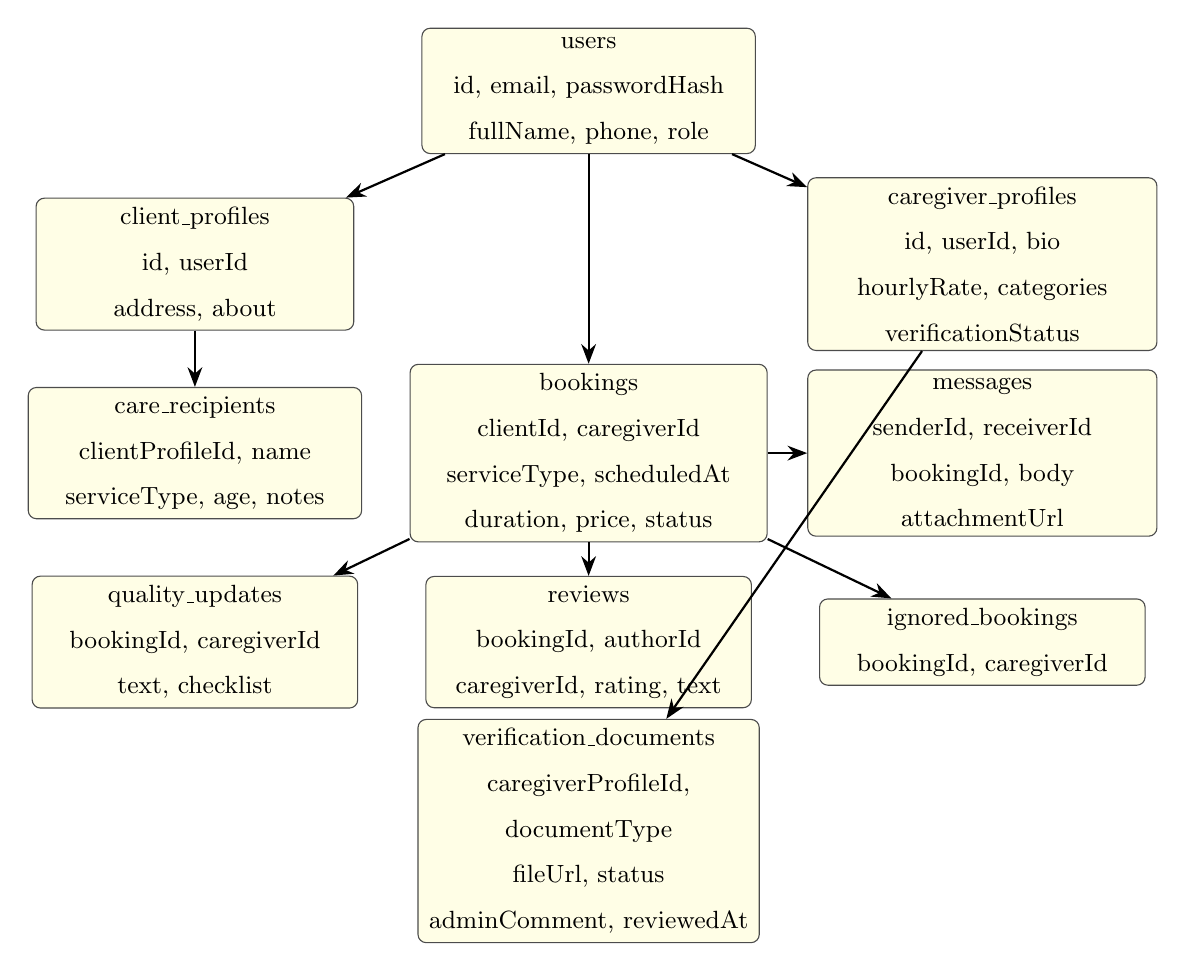
\begin{tikzpicture}[
    entity/.style={rectangle, draw=black!70, rounded corners=3pt, minimum width=3.7cm, minimum height=1cm, align=center, fill=yellow!10, font=\small},
    arr/.style={-{Stealth[length=2.5mm]}, thick}
]
\node[entity, text width=4cm] (users) at (0,0) {users\\id, email, passwordHash\\fullName, phone, role};
\node[entity, text width=3.8cm] (clientp) at (-5,-2.2) {client\_profiles\\id, userId\\address, about};
\node[entity, text width=4.2cm] (caregiverp) at (5,-2.2) {caregiver\_profiles\\id, userId, bio\\hourlyRate, categories\\verificationStatus};
\node[entity, text width=4cm] (recipients) at (-5,-4.6) {care\_recipients\\clientProfileId, name\\serviceType, age, notes};
\node[entity, text width=4.3cm] (bookings) at (0,-4.6) {bookings\\clientId, caregiverId\\serviceType, scheduledAt\\duration, price, status};
\node[entity, text width=4.2cm] (messages) at (5,-4.6) {messages\\senderId, receiverId\\bookingId, body\\attachmentUrl};
\node[entity, text width=3.9cm] (quality) at (-5,-7) {quality\_updates\\bookingId, caregiverId\\text, checklist};
\node[entity, text width=3.9cm] (reviews) at (0,-7) {reviews\\bookingId, authorId\\caregiverId, rating, text};
\node[entity, text width=3.9cm] (ignored) at (5,-7) {ignored\_bookings\\bookingId, caregiverId};
\node[entity, text width=4.1cm] (verdocs) at (0,-9.4) {verification\_documents\\caregiverProfileId, documentType\\fileUrl, status\\adminComment, reviewedAt};

\draw[arr] (users) -- (clientp);
\draw[arr] (users) -- (caregiverp);
\draw[arr] (clientp) -- (recipients);
\draw[arr] (users) -- (bookings);
\draw[arr] (bookings) -- (messages);
\draw[arr] (bookings) -- (quality);
\draw[arr] (bookings) -- (reviews);
\draw[arr] (bookings) -- (ignored);
\draw[arr] (caregiverp) -- (verdocs);
\end{tikzpicture}
}
\caption{Simplified database scheme of the Qamqorshy platform}
\label{fig:qamqorshy-erd}
\end{figure}

The schema also includes one table that supports a small but useful workflow detail: \texttt{ignored\_bookings}. This table allows caregivers to hide open bookings they do not want to accept. Although it is a compact feature from a technical point of view, it improves usability because caregivers do not need to repeatedly dismiss the same request.

\subsubsection{Workflow Design}

The booking workflow was one of the most important parts of the system design because it connects nearly all major features. A client starts by selecting a care category, entering booking details, and optionally choosing a specific caregiver. If no price is entered manually, the backend calculates an initial price using predefined rates for child care, pet care, or elderly care.

Once a booking exists, two different paths are possible. If a caregiver has not been assigned yet, the booking appears in the list of available requests. A caregiver can then accept it or make a counter-offer. If a specific caregiver was already selected, that caregiver can directly respond to the booking. In both cases, negotiation is possible. The caregiver can change the proposed price, and the client can either accept the offer, send another price, or cancel the booking.

Once a caregiver becomes connected to the booking, messaging becomes available between the two participants while the booking remains in an active state. The caregiver can also post quality updates for the assigned booking until it is completed. After completion, the client can leave a review. This flow creates a consistent life cycle for each service request.

The verification workflow is manual by design. The system stores uploaded files and review metadata, while an administrator inspects the submitted documents visually, records a document-level approval or rejection decision, and can still override the caregiver's final verification status through the dedicated administrator endpoint when needed.

\begin{figure}[H]
\centering
\resizebox{0.88\textwidth}{!}{
\begin{tikzpicture}[
    step/.style={rectangle, draw=black!60, rounded corners=4pt, minimum width=4.2cm, minimum height=0.9cm, align=center, fill=blue!5, font=\small},
    decision/.style={diamond, draw=black!60, aspect=2, align=center, fill=orange!8, font=\footnotesize},
    arr/.style={-{Stealth[length=2.5mm]}, thick}
]
\node[step] (start) at (0,0) {Client creates booking};
\node[decision] (assign) at (0,-2) {Specific caregiver selected?};
\node[step] (open) at (-4,-4) {Booking appears in open requests};
\node[step] (direct) at (4,-4) {Booking sent to selected caregiver};
\node[decision] (decision1) at (0,-6.2) {Caregiver accepts or counters?};
\node[step] (accepted) at (-4,-8.4) {Booking accepted};
\node[step] (counter) at (4,-8.4) {Counter-offer sent to client};
\node[decision] (clientdecision) at (4,-10.6) {Client accepts, counters, or cancels};
\node[step] (service) at (0,-12.8) {Active service: messaging and quality updates};
\node[step] (completed) at (0,-15) {Caregiver completes booking};
\node[step] (review) at (0,-17.2) {Client leaves review};

\draw[arr] (start) -- (assign);
\draw[arr] (assign) -- node[above left, font=\footnotesize]{No} (open);
\draw[arr] (assign) -- node[above right, font=\footnotesize]{Yes} (direct);
\draw[arr] (open) -- (decision1);
\draw[arr] (direct) -- (decision1);
\draw[arr] (decision1) -- node[above left, font=\footnotesize]{Accept} (accepted);
\draw[arr] (decision1) -- node[above right, font=\footnotesize]{Counter} (counter);
\draw[arr] (accepted) -- (service);
\draw[arr] (counter) -- (clientdecision);
\draw[arr] (clientdecision) -- node[left, font=\footnotesize]{Accept} (service);
\draw[arr] (service) -- (completed);
\draw[arr] (completed) -- (review);
\end{tikzpicture}
}
\caption{Booking workflow of the Qamqorshy platform}
\label{fig:qamqorshy-booking-workflow}
\end{figure}

\subsubsection{UI Design and Color Palette}

The visual design of Qamqorshy was created to communicate calmness, trust, and warmth. This decision was not accidental. A caregiving platform should not feel like an aggressive marketplace or a cold administrative dashboard. The interface needed to look safe, readable, and inviting because users are making decisions about people who may enter their homes and care for vulnerable family members.

The platform therefore uses a warm palette with soft backgrounds and grounded accent colors. The implementation in the frontend confirms this direction. Repeated use of cream, warm gold, brown, and dark navy creates a balanced visual identity. These colors work well together because they provide contrast without becoming harsh.

\begin{table}[H]
\centering
\caption{Main colors used in the Qamqorshy interface}
\label{tab:colors}
\begin{tabular}{l l l}
\toprule
\textbf{Color name} & \textbf{Hex code} & \textbf{Typical use} \\
\midrule
Warm Gold & \texttt{\#d0a144} & Active highlights, icons, decorative emphasis \\
Soft Brown & \texttt{\#8d6241} & Main buttons, links, secondary accents \\
Deep Navy & \texttt{\#2d3147} & Headings, core text, strong contrast elements \\
Soft Cream & \texttt{\#fffdf9} & Main background areas and cards \\
Light Linen & \texttt{\#f7f1ea} & Section backgrounds and soft contrast blocks \\
Border Sand & \texttt{\#e7dbcf} & Borders, separators, input outlines \\
\bottomrule
\end{tabular}
\end{table}

Typography and spacing also support readability. Large headings and clear section division make the landing page easier to scan. Rounded corners, soft shadows, and moderate whitespace make the platform feel less mechanical. These design choices may seem small on their own, but together they improve comfort and reduce cognitive load for the user.

\begin{figure}[H]
\centering
\fbox{\parbox{0.88\textwidth}{
\centering
\vspace{0.8cm}
\textbf{[Insert Screenshot of Landing Page Here]}\\
\textit{Suggested figure: homepage showing hero section, care categories, and call-to-action blocks.}
\vspace{0.8cm}
}}
\caption{Main landing page of the Qamqorshy platform}
\label{fig:landing-screenshot-placeholder}
\end{figure}

\subsection{Implementation}

\subsubsection{Frontend Implementation}

The frontend of Qamqorshy was implemented as a Next.js application that uses React components and Tailwind CSS for styling. The application follows a page-based structure under the \texttt{app/} directory. Each route corresponds to a user-facing screen such as the landing page, registration page, login page, dashboard, booking form, profile page, messages page, caregiver list, caregiver details, quality updates page, reviews page, and admin panel.

The landing page introduces the platform and explains the available care categories: child care, pet care, and elderly support. The dashboard page adapts its content to the current user role and displays booking lists together with message and review counters. The profile page allows users to edit their information, while caregivers can also define professional fields such as biography, categories, hourly rate, and verification documents.

The frontend communicates with the backend through REST endpoints. It uses helper utilities to fetch data, pass the session token, and render server-side content where appropriate. This structure reduces duplication because page components do not need to hard-code request logic repeatedly. Instead, shared API helpers handle endpoint access.

\subsubsection{Backend Implementation}

The backend was developed with FastAPI because it offers a clean way to define endpoints, validate payloads, and enforce structured response models. The main application file registers route modules for all major parts of the system:

\begin{itemize}[leftmargin=1.5cm]
    \item authentication,
    \item users and dashboards,
    \item profile management,
    \item caregiver listing and verification,
    \item booking management,
    \item messaging,
    \item reviews,
    \item quality updates,
    \item language preference,
    \item administrator statistics,
    \item verification document upload and review.
\end{itemize}

This modular organization reflects the real product domains. Each route file focuses on one area of business logic. For example, the booking module handles creation, listing, available booking retrieval, acceptance, counter-offers, client responses, denial or cancellation, status updates, and single-booking retrieval. The users module exposes current-user data, dashboard aggregation, user lookup, and the list of chat-visible users connected through active assigned bookings. The message module handles text messages and image attachments. The review module enforces the rule that only completed bookings can be reviewed and that each booking can receive only one review from the client. The quality module ensures that only the assigned caregiver can post updates for the relevant booking. The verification-document module handles caregiver uploads, caregiver-side listing and deletion, administrator-side listing, and administrator review decisions.

The backend also uses dependency injection for recurring concerns such as the database session and the current authenticated user. This pattern makes the route handlers shorter and easier to test. More importantly, it keeps security checks consistent across the whole API.

\subsubsection{Authentication and Authorization}

Authentication in Qamqorshy is based on JSON Web Tokens stored in an HTTP-only cookie. When a user registers or logs in successfully, the backend generates a token and sets a session cookie. Because the cookie is HTTP-only, client-side JavaScript cannot read it. That design improves security and reduces the risk of exposing tokens through browser-side scripts.

The registration flow also includes role-sensitive logic. If the new user registers as a caregiver, the backend requires at least one selected category and a valid hourly rate. It then creates a caregiver profile automatically. If the user registers as a client, the backend creates a client profile instead. This design makes onboarding smoother because the account and profile structure are prepared immediately after registration.

Authorization is role-based. The backend checks the current user role before allowing sensitive actions. Only clients can create bookings and leave reviews. Only caregivers can accept bookings, send counter-offers, and upload their verification documents. Only administrators can access system statistics, review uploaded verification documents, and change the caregiver verification status directly. These checks are simple, but they are enforced consistently across the routes.

\subsubsection{Core Functional Features}

The platform includes several main functions that define its practical value. All of them are reflected in the implemented codebase.

\paragraph{1. User Registration and Login.}
The system supports role-based registration for clients and caregivers. During registration, the backend creates the user account, hashes the password, creates the corresponding profile, and signs the user in immediately. Login verifies credentials and issues a fresh token. The authentication module also includes logout, which clears the session cookie.

\paragraph{2. Caregiver Profiles and Verification.}
Caregivers can maintain a profile that includes biography, experience, hourly rate, and service categories. They can also upload identification and qualification files through a dedicated verification section on the profile page. Each uploaded file becomes a separate verification record in the database. Administrators then inspect these files manually, approve or reject them, and can leave a comment explaining the decision. The caregiver's overall verification status is derived from required reviewed documents, while the administrator module still allows a direct status override for operational control.

\paragraph{3. Caregiver Search and Detailed View.}
Clients can browse a list of caregivers and open detailed caregiver pages. The backend enriches caregiver data with reviews and completed job counts. This gives clients more than just a name and price. It gives context, which is exactly what a caregiving platform needs.

\paragraph{4. Booking Creation.}
Clients can create bookings for child care, pet care, or elderly support. A booking includes service type, date and time, duration, notes, optional caregiver selection, tasks, checklist, address, and price. If the client does not enter a price, the backend calculates a default price based on service type and duration.

\paragraph{5. Booking Negotiation.}
One of the strongest functions in the system is price negotiation. A caregiver can accept the proposed booking price or send a counter-offer. The client can then accept, counter again, or cancel the booking. This feature reflects real-world service negotiation instead of forcing a rigid one-price-only model.

\paragraph{6. Available Booking Feed.}
Caregivers can browse open bookings that are not yet assigned. They can filter them by service type. If a caregiver does not want to take a booking, the system can mark it as ignored so it does not reappear unnecessarily. Administrators can also read the available booking feed for monitoring purposes.

\paragraph{7. Booking-Scoped Messaging.}
Messaging is not open-ended. It is tied to active bookings between a client and an assigned caregiver. This was a deliberate design decision. Users can send messages only when they are connected through an active booking. This reduces spam, protects privacy, and keeps communication related to actual service activity. The message module also supports image uploads with file type and file size checks, and the backend exposes a user list built from currently active booking-linked conversations.

\paragraph{8. Quality Updates During Service.}
Caregivers can publish quality updates for bookings assigned to them while those bookings remain unfinished. These updates can include text and checklist information. This function supports trust and transparency, especially when a client wants reassurance that the service is proceeding normally.

\paragraph{9. Reviews and Ratings.}
When a booking reaches the completed state, the client can leave a rating and review text for the caregiver. The system enforces two important rules: the booking must belong to that client, and the client cannot create multiple reviews for the same booking. Reviews later appear on caregiver data shown to users.

\paragraph{10. Role-Based Dashboards.}
The dashboard adapts to the logged-in role. It returns booking data together with message and review counts. For clients, the booking list is limited to their own requests. For caregivers, it shows their assigned work. For administrators, it can expose the full booking list. This gives each user a practical summary instead of forcing them to visit many separate pages for basic information.

\paragraph{11. Administrator Panel.}
The admin panel displays total user count, booking count, and review count. It also shows the caregiver verification area, where administrators can inspect uploaded verification documents, leave review comments, update the document status to approved or rejected, and, through a separate administrative route, update the caregiver's overall verification status directly.

\paragraph{12. Multilingual Support.}
The platform includes language selection logic and stores the chosen language in cookies. The backend accepts only the supported locales Kazakh, Russian, and English, then writes both \texttt{lang} and \texttt{NEXT\_LOCALE} cookies. This keeps the behavior predictable across the interface. It is especially important in Kazakhstan, where users may expect to interact with the system in Kazakh, Russian, or English. Multilingual support also improves accessibility and professionalism.

\begin{figure}[H]
\centering
\fbox{\parbox{0.88\textwidth}{
\centering
\vspace{0.8cm}
\textbf{[Insert Screenshot of Dashboard Here]}\\
\textit{Suggested figure: role-based dashboard with booking, message, and review counters.}
\vspace{0.8cm}
}}
\caption{Dashboard interface of the Qamqorshy platform}
\label{fig:dashboard-placeholder}
\end{figure}

\begin{figure}[H]
\centering
\fbox{\parbox{0.88\textwidth}{
\centering
\vspace{0.8cm}
\textbf{[Insert Screenshot of Booking Page Here]}\\
\textit{Suggested figure: booking form or booking management page with care type and price information.}
\vspace{0.8cm}
}}
\caption{Booking creation and management interface}
\label{fig:booking-placeholder}
\end{figure}

\begin{figure}[H]
\centering
\fbox{\parbox{0.88\textwidth}{
\centering
\vspace{0.8cm}
\textbf{[Insert Screenshot of Messages or Quality Updates Here]}\\
\textit{Suggested figure: booking-scoped chat or quality update timeline.}
\vspace{0.8cm}
}}
\caption{Communication and service monitoring features}
\label{fig:communication-placeholder}
\end{figure}

\subsubsection{Security and Data Integrity}

Security decisions in Qamqorshy were directly connected to the nature of the platform. Because the application handles personal information, messages, and care-related details, it needed basic but reliable protection mechanisms.

Passwords are hashed with bcrypt before they are stored in the database. Tokens are kept in an HTTP-only cookie. API payloads are validated with Pydantic. Route handlers check role permissions before performing sensitive actions. Database foreign keys preserve relational consistency between users, profiles, bookings, messages, and reviews. Together, these decisions create a system that is much safer than a simple prototype with plain text credentials or unvalidated input.

Validation also protects the operational logic of the platform. For example, booking requests require a future date and a positive duration, caregiver registration requires at least one category and a positive hourly rate, review text must contain meaningful content, quality updates cannot be blank, and verification review requests must use valid document statuses. These rules reduce the chance of inconsistent or misleading data entering the system.

The application also applies functional integrity rules. Messages can only be exchanged between users linked by an active booking. Reviews can only be added after completion. Quality updates can only be posted by the caregiver assigned to the booking. Those rules are not only business logic; they are also part of keeping the data meaningful and trustworthy.

\subsubsection{Testing and Validation}

Testing was performed continuously during development rather than only at the end. The team checked backend endpoints by sending requests for normal and edge cases, such as invalid login data, missing required fields, forbidden role actions, and incorrect booking transitions. The frontend was tested by navigating through the main pages, checking role-specific rendering, verifying page access control, and confirming that data from the API appeared correctly in the interface.

Special attention was given to the full service flow because this is where many independent modules meet. A typical validation scenario included registering a user, signing in, creating a booking, accepting or negotiating it as a caregiver, sending messages, posting quality updates, completing the booking, and then leaving a review. This end-to-end validation was important because isolated page checks cannot reveal every integration issue.

\subsection{Chapter Summary}

This chapter presented the design and methodology of the Qamqorshy platform from problem definition to implementation details. The project began with a clear market gap in Kazakhstan: the absence of a dedicated digital platform for caregiving services. Existing marketplaces offered only limited and overly general caregiver listings, which did not provide enough trust or specialization for real caregiving needs. In response, the team designed and developed Qamqorshy as a focused platform for child care, pet care, and elderly support.

The chapter described the Agile development process, the selected architecture, the technology stack, the project structure, the database schema, the main workflows, the visual design logic, and the major functional modules implemented in the system. The result is a platform that combines role-based access, structured booking, negotiation, communication, verification, reviews, and multilingual support in one coherent environment.

\bigskip
\noindent\textbf{Markers to replace later:}
\begin{itemize}[leftmargin=1.5cm]
    \item \textbf{[Insert Team Name Here]}
    \item \textbf{[Insert Project Management Tool Here]}
    \item \textbf{[Insert Communication Tool Here]}
    \item \textbf{[Insert Screenshot of Landing Page Here]}
    \item \textbf{[Insert Screenshot of Dashboard Here]}
    \item \textbf{[Insert Screenshot of Booking Page Here]}
    \item \textbf{[Insert Screenshot of Messages or Quality Updates Here]}
\end{itemize}

\end{document}
